\documentclass[../DS06.tex]{subfiles}
\graphicspath{{./figures/}}

% \subimport{/home/nora/Documents/Enseignement/Prepa/bpep/exercices/DS/HP_electrostatique/}{sujet.tex}

\begin{document}
\exercice[21]{Toboggans\ifcorrige{~\small\textit{(D'après CCS TSI 2018)}}}

\enonce{
	\noindent
	\begin{minipage}[c]{.45\linewidth}
		Les toboggans font aujourd'hui partie des incontournables d’un centre
		aquatique. De nombreux toboggans présentent des enroulements plus ou moins
		complexes.
		\bigbreak
		On étudie le toboggan présenté ci-contre et composé d’un enroulement
		hélicoïdal d’approximativement $n = \num{2,3}$ tours. Le rayon moyen est
		estimé à $R = \SI{2,0}{\metre}$ et la hauteur de l’ensemble est $h =
			\SI{4}{\metre}$.
		\bigbreak
		On néglige les frottements. On note $\th > 0$ la position angulaire d'une
		baigneuse dans le toboggan relativement à la position de départ, d’altitude
		$h$.
	\end{minipage}
	\hfill
	\begin{minipage}[c]{.45\linewidth}
		~
		\begin{center}
			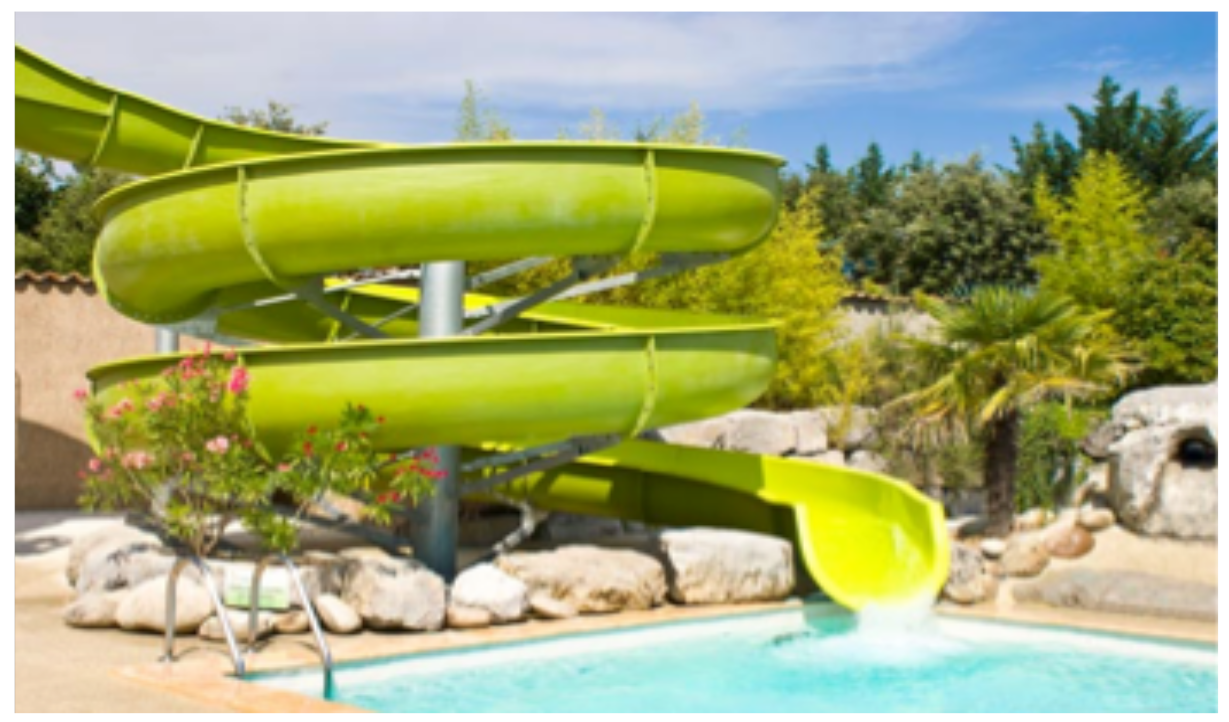
\includegraphics[width=\linewidth]{toboggan}
			\captionof{figure}{Illustration.}
			\label{fig:toboggan}
		\end{center}
	\end{minipage}
	Une baigneuse de masse $m$ suit la trajectoire d’équation $r = R$, $z =\alpha
		\th$, l’axe $(z'z)$ étant orienté selon la \textbf{verticale descendante}.
}

\QR[2]{%
	Déterminer la valeur de $\alpha$.
}{%
	\vspace{-15pt}
	\[
		h = z_{\max} \Lra h = \alpha \times n \times 2\pi
		\Lra
		\boxed{\alpha \stm{=} \frac{h}{2\pi n}}
		\Lra
		\xul{\alpha \stm[-1]{=} \SI{0,28}{\metre\per\radian}}
	\]
}

\QR[2]{%
	Sachant qu'on oriente l'axe vertical descendant, quelle est l'expression
	générale de l'énergie potentielle de pesanteur $\Ec_{p,p}$ en fonction de
	$z$~?
}{%
	L'énergie doit diminuer quand $z$ augmente \pt{1} (de haut en bas), donc
	\[
		\boxed{\Ec_{p,p} \stm[-1]{=} -mgz + \stm[-1]{\cte}}
	\]
}

\QR[4]{%
	Calculer la valeur de la vitesse atteinte en sortie du toboggan, le départ se
	faisant sans vitesse initiale.
}{%
	Les frottements sont négligés, donc l'énergie mécanique $\Ec_m$ se conserve
	\pt{1}~:
	\begin{align*}
		\Ec_{m,\rm init}    & \stm[-1]{=} \Ec_{m,\rm fin}
		\\
		\beforetext{Or}
		\Ec_{m,\rm init} = \frac{1}{2} mv_{\rm init}^2 -mgz_{\rm init} = 0 + 0
		\qquad              & \stm[-1]{\text{et}} \qquad
		\Ec_{m,\rm fin} = \frac{1}{2} mv_{\rm fin}^2 -mgh
		\\\Lra
		\Aboxed{v_{\rm fin} & \stm[-1]{=} \sqrt{2gh}}
	\end{align*}
}

\enonce{
	Afin d’éviter d’éventuelles collisions, le toboggan est équipé au point de
	départ d’un feu qui passe au vert toutes les $t_f$ secondes. On impose une
	marge de $t_m = \SI{5}{\second}$ en plus de la durée de parcours dans le
	toboggan.
}

\QR[2]{%
	Exprimer le vecteur vitesse dans la base cylindrique en fonction de $R$,
	$\alpha$ et $\tp$.
}{%
	Le vecteur position est (avec les notations habituelles)~:
	\begin{gather*}
		\OM \stm[-1]{=} R\er + z\ez \Lra \OM = R\er + \alpha \th \ez
		\\\Lra
		\boxed{\vv{v} \stm{=} R \tp \et + \alpha \tp \ez}
	\end{gather*}
}

\QR[2]{%
	Exprimer l'énergie mécanique de la baigneuse en fonction de $m$, $g$, $R$,
	$\alpha$ et $\tp$.
}{%
	\vspace{-15pt}
	\begin{gather*}
		\Ec_c = \frac{1}{2} m v^2 \stm[-1]{=}
		\frac{1}{2} m \left[(R \tp)^2 + (\alpha \tp)^2 \right]
		\qet
		\Ec_p = -mgz + K \stm[-1]{=} -mg\alpha \th +K.
		\\\Ra
		\boxed{
			\Ec_m = \frac{1}{2} m \left[(R \tp)^2 +
				(\alpha \tp)^2 \right] -mg\alpha \th +K
		}
	\end{gather*}
}

\QR[6]{%
	Dériver cette expression et en déduire, après résolution de l'équation
	obtenue, l'expression de $\th (t)$.
}{%
	Puisqu'il n'y a pas de frottement, l'énergie mécanique se conserve dans le
	temps, donc $\dd\Ec_m/\dt = 0$ \pt{1}~:
	\begin{DispWithArrows*}
		\dv{\Ec_m}{t} = 0
		\Lra
		m \big[(R^2 \tp \tpp) &+ (\alpha^2 \tp \tpp) \big] -mg\alpha \tp = 0
		\Arrow{$\tp \neq 0$ constamment}
		\\\Lra
		\Aboxed{
			(R^2+\alpha^2)&\tpp -g\alpha \stm[-1]{=} 0
		}
	\end{DispWithArrows*}
	\vspace{-15pt}
	\begin{gather*}
		\beforetext{On trouve~:}
		\tpp = \frac{g\alpha}{R^2+\alpha^2}
		\quad \Rightarrow \quad
		\tp = \frac{g\alpha}{R^2+\alpha^2}t + K_1
		\quad \Rightarrow \quad
		\th(t) \stm{=} \frac{g\alpha}{2(R^2+\alpha^2)}t^2 + K_1t + K_2.
	\end{gather*}
	On peut trouver les valeurs des constantes d'intégrations en utilisant les
	conditions initiales~:
	\begin{gather*}
		\tp(0)=0
		\quad
		\th (0)=0
		\quad \Rightarrow \quad
		K_1=K_2=0 \pt{1}
		\\\Ra
		\boxed{\th(t) \stm{=} \frac{g\alpha}{2(R^2+\alpha^2)}t^2}.
	\end{gather*}
}

\QR[3]{%
	Calculer $t_f$. On prendra $g = \SI{9,8}{\metre\per\second^2}$.
}{%
	\vspace{-15pt}
	\begin{gather*}
		\beforetext{En inversant la relation précédente~:}
		\boxed{t \stm{=} \sqrt{\frac{2\th (R^2+\alpha^2)}{g\alpha}}}
	\end{gather*}
	La valeur de $\th$ lorsque la baigneuse sort du toboggan est $\th_{\rm max} =
		2\pi \times n$. On a alors~:
	\[
		\boxed{t_f \stm{=} t_m + \sqrt{\frac{4n\pi(R^2+\alpha^2)}{g\alpha}}}
		\Lra
		\xul{t_f \stm[-1]{=} \SI{11,5}{\second}}
		\qav
		\left\{
		\begin{array}{rcl}
			n      & = & \num{2.3}
			\\
			R      & = & \SI{2.0}{m}
			\\
			\alpha & = & \SI{0.28}{rad.s^{-1}}
			\\
			g      & = & \SI{9.8}{m.s^{-2}}
		\end{array}
		\right.
	\]
}

\end{document}
